% Created 2016-08-17 Wed 14:38
\documentclass[tikz]{standalone}

\usepackage[utf8]{inputenc}
\usepackage[T1]{fontenc}

\usepackage{circledsteps}

\RequirePackage{xcolor}

%% HPI color definitions according to the design manual
% These do not exactly match the RGB values used in the Powerpoint slide master due to unknown reasons
\definecolor{hpiyellow}{RGB}{246,168,0}
\definecolor{hpiorange}{RGB}{221,97,8}
\definecolor{hpired}{RGB}{177,6,58}
\definecolor{hpigray}{RGB}{90,96,101}
\definecolor{hpiblue}{RGB}{0,122,158}


\renewcommand{\sfdefault}{neosans}
% Different font weights for neosans
\newcommand{\textl}[1]{{\fontseries{l}\selectfont #1}} % light
\newcommand{\textm}[1]{{\fontseries{m}\selectfont #1}} % medium, same as default weight
\newcommand{\textsb}[1]{{\fontseries{sb}\selectfont #1}} % semibold
\newcommand{\textmb}[1]{{\fontseries{mb}\selectfont #1}} % bold, same as \textbf
\newcommand{\texteb}[1]{{\fontseries{eb}\selectfont #1}} % extra bold
\newcommand{\textub}[1]{{\fontseries{ub}\selectfont #1}} % ultra bold

\tikzset{every picture/.style={/utils/exec={\sffamily}}}
\tikzset{flipflop RSflanke/.style={
  flipflop,
  flipflop def={t1=S, t2=C, c2=1, t3=R, t6=Q, t4={\ctikztextnot{Q}}}
}}


\tikzset{
  mechanicalSwitch/.pic={
    \coordinate (-inUp) at (135:2); 
    \coordinate (-inDown) at (235:2);
    \coordinate (-out) at (2,0);
    \coordinate (-center) at (0,0);
    
    \draw (0,0) circle [radius = 2cm];
    \draw [fill=gray!20] (0,0) circle [radius = 0.2cm];

    \draw (0, 0) -- (2, 0);
    \draw (135:.8) -- (135:2); 
    \draw (225:.8) -- (225:2); 

    \draw [fill=gray!20] (2, 0) circle [radius=0.05cm]; 
    \draw [fill=gray!20] (135:2) circle [radius=0.05cm]; 
    \draw [fill=gray!20] (225:2) circle [radius=0.05cm]; 

    
    \draw [thick] (0,0) -- (175:1.5); 

    \draw [dashed, <->, domain=135:225] plot ({cos(\x)}, {sin(\x)}); 
  },
  mechanicalSwitchClosed/.pic={
    \coordinate (-inUp) at (135:2); 
    \coordinate (-inDown) at (255:2);
    \coordinate (-out) at (2,0);
    \coordinate (-center) at (0,0);
    \draw (0,0) circle [radius = 2cm];
    \draw [fill=gray!20] (0,0) circle [radius = 0.2cm];

    \draw (0, 0) -- (2, 0);
    \draw (135:.8) -- (135:2); 
    \draw (225:.8) -- (225:2); 

    \draw [fill=gray!20] (2, 0) circle [radius=0.05cm]; 
    \draw [fill=gray!20] (135:2) circle [radius=0.05cm]; 
    \draw [fill=gray!20] (225:2) circle [radius=0.05cm]; 

    
    \draw [thick] (0,0) -- (135:2); 

    \draw [dashed, <->, domain=135:225] plot ({cos(\x)}, {sin(\x)}); 
  }
}


\usetikzlibrary{calc}
\usetikzlibrary{positioning}


\usetikzlibrary{decorations.pathreplacing}


\begin{document}


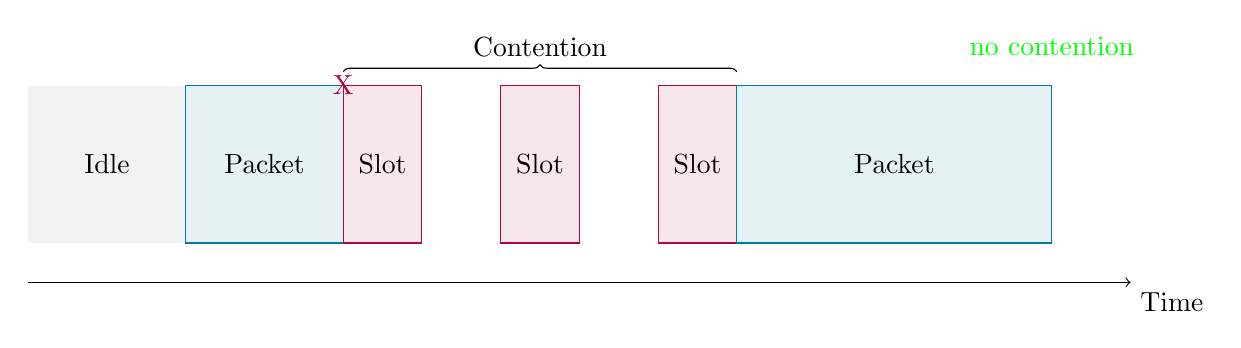
\begin{tikzpicture}
  \label{page:mac:contentionslots}
  
  \draw [->] (0,0.5) -- ++(14,0) node [below right] {Time};

  % \node [fill=gray!10] ()
  \draw [fill=gray!10,draw=none] (0,1) rectangle node{Idle} (2,3);
  \draw [fill=hpiblue!10,draw=hpiblue] (2,1) rectangle node{Packet} (4,3);
  \draw [fill=hpired!10,draw=hpired] (4,1) rectangle node{Slot} (5,3);
  \draw [fill=hpired!10,draw=hpired] (6,1) rectangle node{ Slot} (7,3);
  \draw [fill=hpired!10,draw=hpired] (8,1) rectangle node{ Slot} (9,3);
  \node [hpired] at (4,3) {\textbf{X}};

  
  \draw [fill=hpiblue!10,draw=hpiblue] (9,1) rectangle node{Packet} (13,3);
  \node [green] at (13,3.5) {\textbf{no contention}};

  \draw [decorate,decoration={brace, raise=5pt}] (4,3) to node[above=0.25cm] {Contention} (9,3); 
  
\end{tikzpicture}


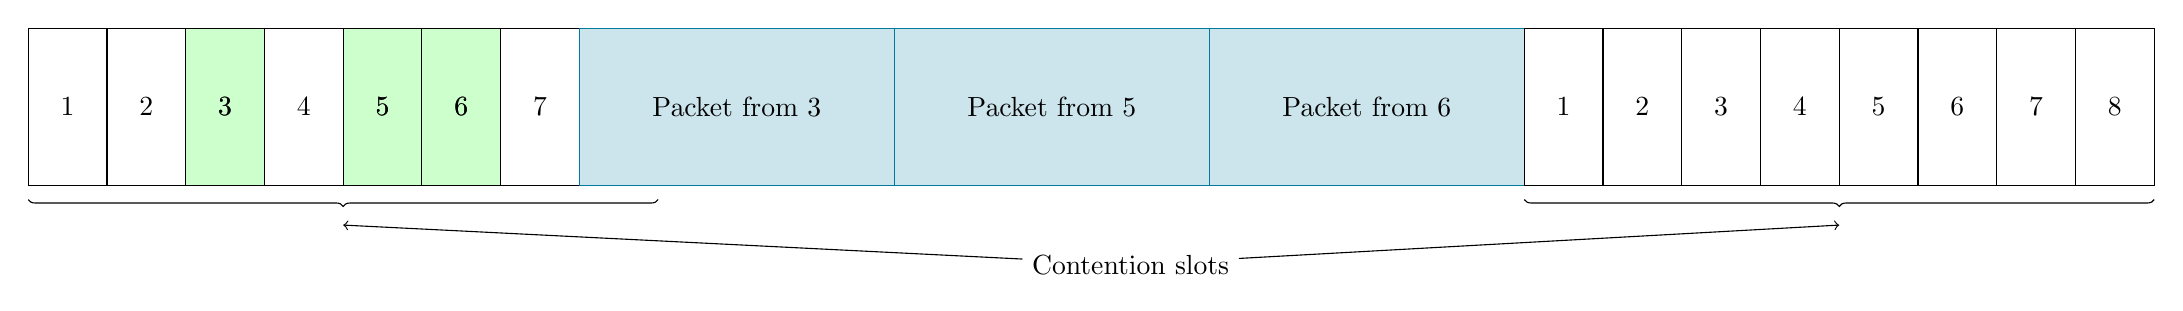
\begin{tikzpicture}
  \label{page:mac:bitmap}
  \foreach \i in {3,5,6} {
    \draw [fill=green!20] (\i,0) rectangle node {\i} (\i+1,2); 
  }
  
  \foreach \i in {1,...,8} {
    \draw (\i,0) rectangle node {\i} (\i+1,2); 
  }

  \foreach \i [count=\ci] in {3,5,6} {
    \draw [fill=hpiblue!20,draw=hpiblue] (4+4*\ci,0) rectangle node {Packet from \i} (4+4*\ci +4, 2); 
  }

  \foreach \i in {1,...,8} {
    \draw (20+\i-1,0) rectangle node {\i} (20+\i+1-1,2); 
  }

  \draw [decorate, decoration={brace, raise=5pt, mirror}] (1,0) to node (cs1) {} (9,0); 
  \draw [decorate, decoration={brace, raise=5pt, mirror}] (20,0) to node (cs2) {} (28,0); 
  \node at (15,-1) (cslabel){Contention slots}; 

  \draw [->] (cslabel) -- (5, -0.5); 
  \draw [->] (cslabel) -- (24, -0.5); 
\end{tikzpicture}

\end{document}

